\documentclass[a4paper,12pt]{article} % тип документа
\usepackage[margin=1in]{geometry} % Поля

%  Русский язык
\usepackage[warn]{mathtext}
\usepackage[T2A]{fontenc}			% кодировка
\usepackage[utf8]{inputenc}			% кодировка исходного текста
\usepackage[english,russian]{babel}	% локализация и переносы
% Математика
\usepackage{amsmath,amsfonts,amssymb,amsthm,mathtools} 
\usepackage{wasysym}
%%%
\usepackage{graphicx}

\usepackage{tabularx}

\usepackage{gensymb} % знак градуса
\usepackage{enumitem} % изменить список enumerate
\usepackage{placeins} % \FloatBarrier

\renewcommand{\thesection}{\Roman{section}} 
\renewcommand{\thesubsection}{\roman{subsection}}
\renewcommand{\thesubsubsection}{\roman{subsection}.\roman{subsubsection}}


\begin{document}

\newcolumntype{Y}{>{\centering\arraybackslash}X} %new tabularx


%титул
\hrule 	
\medskip
\begin{raggedright}
{\large \textbf{Отчёт по работе 4.1.1}}
\\
\medskip
{\Large Изучение центрированных оптических систем} 
\\
\medskip
{\large Карташов Констанин Б04-005}
\medskip
\hrule
\medskip
\end{raggedright}


\section{Анотация}

\paragraph{Цель работы:} 
Изучит методы определения фокусных расстояний линз и сложных оптических систем; определить характеристики оптической систем, составленной из тонких линз, изучить недостатки реальных линз -- сферическую и хроматическую аберрации.

\paragraph{Оборудование:}
\begin{itemize}
\renewcommand{\labelitemi}{$\triangleright$}
\itemsep0em
\item Оптическая скамья с набором рейтеров
\item Положительные и отрицательные линзы
\item Экран
\item Осветитель с ирисовой диафрагмой
\item Зрительная труба 
\item Светофильтры
\item Кольцевые диафрагмы
\item Линейка
\end{itemize}


\medskip\hrule\medskip

\section{Теоретическая часть}

\subsection{Определение фокусного расстояния оптических систем по методу Аббе}

\begin{figure}[h]
\centering
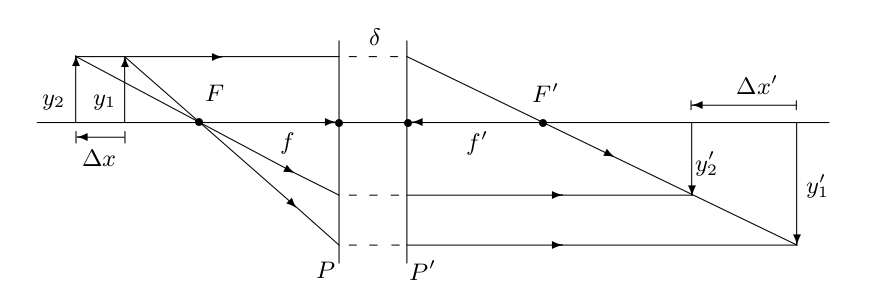
\includegraphics[width=\textwidth]{abbe.png}
\caption{Метод Аббе}
\label{fig:abbe}
\end{figure}

\paragraph{} Измерение фокусного расстояния по методу Аббе основано на определении поперечного увеличения для нескольких (не менее двух) различных положений предмета, находящегося на оптической оси исследуемой оптической системы. На рис. \ref{fig:abbe} представлена соответствующая схема эксперимента. Фокусное расстояние системы можно выразить через положения предмета и соответствующие увеличения следующим образом:

\begin{equation}
f = \frac{\Delta x}{\Delta(y/y')} = - \frac{\Delta x'}{\Delta(y'/y)}
\label{e:abbe}
\end{equation}

\subsection{Определение фокусного расстояния оптических систем по методу Бесселя}

\begin{figure}[h]
\centering
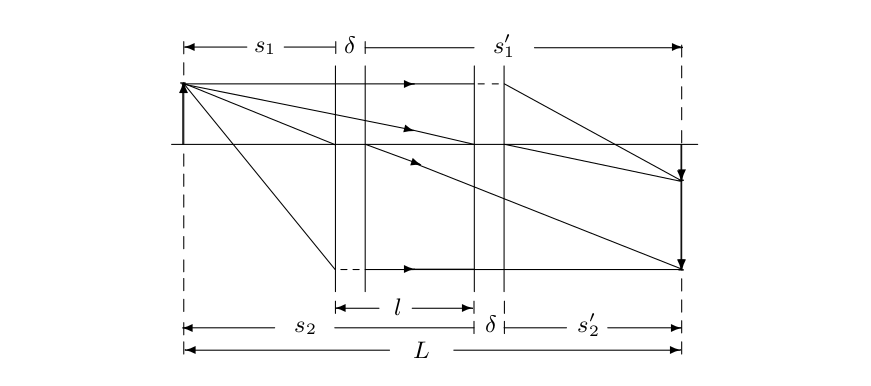
\includegraphics[width=\textwidth]{bessel.png}
\caption{Метод Бесселя}
\label{fig:bessel}
\end{figure}

\paragraph{} Схема метода Бесселя для случая, когда $n = n'$ и $f' = -f$ , представлена на рис. \ref{fig:abbe}. Она основана на том, что при заданном расстоянии $L$ между предметом и экраном выполняется соотношение, представляющее собой квадратное уравнение относительно расстояния $s$ от главной плоскости пространства предметов до предмета ($s < 0$):

\begin{equation}
-\frac{1}{s} + \frac{1}{L - \delta + s} = \frac{1}{f},
\label{e:bessel1}
\end{equation}

\noindent имеющее при условии $L > 4f + \delta$ решения $s1$ и $s2$ , показанные на рис. \ref{fig:bessel}, где $\delta$ — расстояние между главными плоскостями системы (линзы).

\paragraph{} Решив уравнение можно получить соотношение:

\begin{equation}
f = \frac{(L - \delta)^2 - l^2}{4(L - \delta},
\label{e:bessel2}
\end{equation}

\noindent которое при условии $|\delta| \ll L$ можно упростить до вида:

\begin{equation}
f = \frac{L^2 - l^2}{4L}
\label{e:bessel}
\end{equation}

\subsection{Определение фокусного расстояния тонкой рассеивающей линзы}

\begin{figure}[h]
\centering
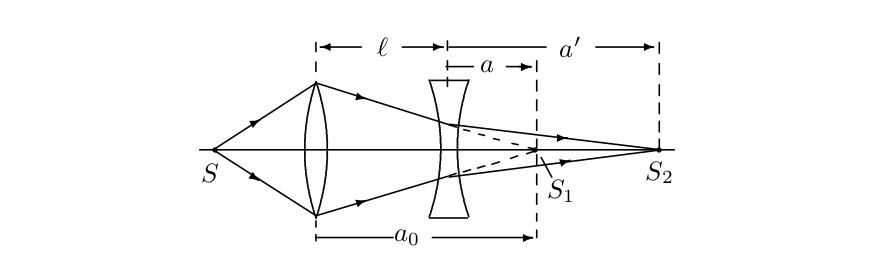
\includegraphics[width=\textwidth]{rass.png}
\caption{Определение фокусного расстояния тонкой рассеивающей линзы}
\label{fig:rass}
\end{figure}

Сначала с помощью собирающей линзы получают на экране действительное изображение предмета S (точка $S_1$ на рис. \ref{fig:rass}). Затем на пути лучей, выходящих из собирающей линзы, располагают исследуемую рассеивающую линзу и, отодвигая экран, получают чёткое изображение предмета на экране, образованное двумя линзами. Определив расстояния $a = a_0 - l > 0$ и $a' > 0$, рассчитывают фокусное расстояние рассеивающей линзы по формуле:

\begin{equation}
-\frac{1}{a} 	+ \frac{1}{a'} = \frac{1}{f}
\label{e:rass}
\end{equation}

\medskip\hrule\medskip

\FloatBarrier

\section{Экспериментальная часть}

\subsection{Определение фокусных расстояний тонких линз при помощи экрана}

\subsubsection{Метод Аббе}

\paragraph{} Измерим фокусное расстояние центрированной линзы №1 методом Аббе. Получим изображение на экране, затем переместим экран и осветитель и получим изображение другого размера. Далее по формуле (\ref{e:abbe}) найдём фокусное расстояние линзы:

\[
\begin{array}{llll}
y = 2 \text{ см}, 	& x_1 = 13 \text{ см},	& x_1' = 53 \text{ см}, & y_1' = 8.5 \text{ см}, \\
 - 					& x_2 = 17 \text{ см},	& x_2' = 25 \text{ см}, & y_2' = 3 \text{ см}, \\
\end{array}
\]

\[
f_1 = \frac{17 - 13}{\frac{2}{3} - \frac{2}{8.5}} \approx 9.27, \;\;\;
f_1' = \frac{25 - 53}{\frac{3}{2} - \frac{8.5	}{2}} \approx 10.18.
\]

\noindent Среднее $f_1 = 9.73$ см.

\paragraph{} Погрешность измерений методом Аббе будет складывается из погрешностей измерения $x_1, x_2, x_1', x_2'$ (если считать, что значение $y$ нам дано) это может даль особенно сильную погрешность, если числа в знаменателе малы.

\subsubsection{Метод Бесселя}

\paragraph{} Измерим фокусное расстояние центрированной линзы №1 методом Бесселя. Проведём несколько измерений и найдём среднее и случайную погрешность. Результаты измерений и вычислений внесём в таблицу \ref{tab:bessel}.

\paragraph{} По значения для $f_1$ из табл. \ref{tab:bessel} вычислим среднее и случайную погрешность (среднеквадратичное отклонение): $\bar{f_1} = 10.13,\; \sigma_{f_1} = 0.10$.

\begin{table}[]
\centering
\begin{tabular}{|l|l|l|l|l|l|l|l|}
\hline
№ изм. & $a_1$, см & $a_1'$, см & $a_2$, см & $a_2$', см & $L$, см & $l$, см & $f_1$, см \\ \hline
1      & 18        & 23.5       & 24        & 17.5       & 41.5    & 6       & 10.16     \\ \hline
2      & 15        & 30         & 29        & 16         & 45      & 14      & 10.16     \\ \hline
3      & 14        & 36         & 35        & 14         & 49.5    & 21.5    & 10.04     \\ \hline
4      & 14        & 42         & 41.5      & 13.5       & 55.5    & 28      & 10.34     \\ \hline
5      & 12        & 57         & 57        & 12.5       & 69.25   & 44.75   & 10.08     \\ \hline
6      & 11.5      & 78         & 78        & 11.5       & 89.5    & 66.5    & 10.02     \\ \hline
7      & 13        & 45         & 45        & 13         & 58      & 32      & 10.09     \\ \hline
\end{tabular}
\caption{Измерения фокусного расстояния по методу Бесселя}
\label{tab:bessel}
\end{table}

\subsubsection{Рассеивающая линза}

\paragraph{} Измерим фокусное расстояние рассеивающей линзы. Для это сначала получим изображение на экране при помощи собирающей линзы, и измерим расстояние $a_0$, а затем отдалим изображение рассеивающей линзой и измерим расстояния $l$ и $a'$ (рис. \ref{e:rass}). Затем по формуле (\ref{e:rass}) определим фокусное расстояние рассеивающей линзы $f_-$. Получаем:

\[
a_0 = 14.5 \text{ см}, \; a' = 13.5 \text{ см}, \; l = 8 \text{ см} \; \Rightarrow \; a = 6.5 \text{ см}, \; f_- = \frac{aa'}{a-a'} \approx -12.5 \text{ см}.
\]

\subsection{Определение фокусных расстояний тонких линз с помощью зрительной трубы}

\subsubsection{Линза №1}

\paragraph{} Расположим на оптическом столе осветитель, линзу №1 и зрительную трубу, предварительно настроенную на бесконечность. Получим чёткое изображение осветителя в зрительной трубе, и измерим расстояние от линзы до осветителя. Затем перевернём линзу и повторим опыт. В качестве фокусного расстояния возьмём среднее значение. Получили: $f_1^1 = 10.3$ см , $f_1^2 = 10.5$ см, $f_1 = 10.4$ см.

\subsubsection{Линза №2}

\paragraph{} Проведём такой же опыт для линзы №2. Получим: $f_2^1 = 13.1$ см, $f_2^2 = 13.3$ см, $f_2 = 13.2$ см.

\paragraph{} Погрешность измерения фокусного расстояния линзы при помощи зрительной трубы можно оценить как погрешность двух измерений линейкой ($\sigma_f \approx 1$ мм), однако это не учитывает особенностей глаза наблюдателя и того, что изображение может быть чётким в некотором интервале. Полученные значения занесём в таблицу \ref{tab:dptr}

\begin{table}[]
\centering
\begin{tabular}{|l|l|l|}
\hline
Линза & $f$, см & $D$, дптр\$ \\ \hline
№1    & 10.4    & 9.6         \\ \hline
№2    & 13.2    & 7.6         \\ \hline
расс. & 12.5    & -8          \\ \hline
\end{tabular}
\caption{Измеренные фокусные расстояния и оптические силы линз}
\label{tab:dptr}
\end{table}

\subsection{Определение фокусного расстояния и положения главных и фокальных плоскостей сложной оптической системы}

\subsubsection{Измерение фокусного расстояния по методу Аббе}

\paragraph{} Соберём сложную систему из линзы №1 и №2, расположенных на расстоянии $l_{12} = 5.5$ см. Далее по методу Аббе найдём фокусное расстояние:

\[
\begin{array}{llll}
y = 2 \text{ см}, 	& x_1 = 5.8 \text{ см},	& x_1' = 39.5 \text{ см}, & y_1' = 10 \text{ см}, \\
 - 					& x_2 = 9.1 \text{ см},	& x_2' = 15 \text{ см}, & y_2' = 3 \text{ см}, \\
\end{array}
\]

\[
f_\Sigma = \frac{9.1 - 5.8}{\frac{2}{3} - \frac{2}{10}} \approx 7.07, \;\;\;
f_\Sigma' = \frac{15 - 39.5}{\frac{3}{2} - \frac{10}{2}} = 7.
\]

\noindent Среднее $f_\Sigma = 7.03$ см.

\subsubsection{Нахождение главных фокусов системы}

\paragraph{} Расположим зрительную трубу за сложной системой, и передвигая осветитель за линзой №1, добьёмся чёткого изображения в зрительной трубе. Измерив расстояние от линзы №1 до осветителя получим положения главного фокуса $F_{\Sigma 1} = 4.6$ см.

\paragraph{} Тоже самое повторим для линзы №2. Получим $F_{\Sigma 2} = 4.0$ см.

\paragraph{} Для погрешностей измерений фокусного расстояния и главных фокусов справедливы рассуждения для погрешностей измерений методом Аббе и зрительной трубой.

\subsubsection{Построение геометрической модели сложной системы} 

\paragraph{} Построим модель сложной системы на миллиметровой бумаге (прил. 1). Построим падающие на систему слева и справа лучи параллельные оптической оси. По рисунку рассчитаем: $f_\Sigma = 7.6$ см, $H_{1\Sigma} = 3.2$ см, $H_{2\Sigma} = 4.0$ см, $F_{1\Sigma} = 4.4$ см, $F_{2\Sigma} = 3.6$ см.

\paragraph{} Также рассчитаем эти значения исходя из формул:

\[
H_{1\Sigma} = \frac{f_1 l_{12}}{l_{12} - f_1 - f_2} = 3.16 \text{ см}, \; H_{2\Sigma} = \frac{f_2 l_{12}}{l_{12} - f_1 - f_2} = 4.01 \text{ см},
\]\[
F_{1\Sigma} = f_1\left( 1 + \frac{f_1}{l_{12} - f_1 - f_2}\right) = 4.42 \text{ см}, \; F_{2\Sigma} = f_2\left( 1 + \frac{f_2}{l_{12} - f_1 - f_2}\right) = 3.57 \text{ см},
\]\[
f_\Sigma = \frac{f_1 f_2}{l_{12} - f_1 - f_2} = 7.58 \text{ см}.
\]

\paragraph{} Все значения занесём в таблицу \ref{tab:ways}:

\begin{table}[h]
\centering
\begin{tabular}{|l|l|l|l|l|l|}
\hline
Способ & $f$, см & $F_{1\Sigma}$, см & $F_{2\Sigma}$, см & $H_{1\Sigma}$, см & $H_{2\Sigma}$, см \\ \hline
Измерение  & 7.0  & 4.6  & 4.0  & --   & --   \\ \hline
Построение & 7.6  & 4.4  & 3.6  & 3.2  & 4.0  \\ \hline
Формулы    & 7.57 & 4.42 & 3.57 & 3.16 & 4.01 \\ \hline
\end{tabular}
\caption{Значения для параметров сложной системы полученные разными способами}
\label{tab:ways}
\end{table}

\subsection{Основные аберрации оптических систем}

\subsubsection{Сферическая аберрация}

\paragraph{} Последовательно перекрывая линзу №3 диафрагмами различных диаметров $2h$, измерим соответствующие фокусные расстояния $s$:

\begin{table}[h]
\centering
\begin{tabular}{|l|l|l|l|}
\hline
$h$, см & 0.5 & 1 & 2   \\ \hline
$s$, см & 7.2 & 7 & 6.2 \\ \hline
\end{tabular}
\caption{Наблюдения сферической аберрации}
\label{tab:shpere}
\end{table}

\paragraph{} Построим график $s(h^2)$ по точкам из табл. \ref{tab:shpere} (рис. \ref{fig:shpere}). Точки на графике лежат на одной прямой, экстраполируем эту прямую до точек $h = 0$ и $h = r$, и рассчитаем продольную сферическую аберрацию линзы $\delta s = s(r) - s(0) = 4.867 - 7.267 = -3.6$ см.

\begin{figure}
\centering
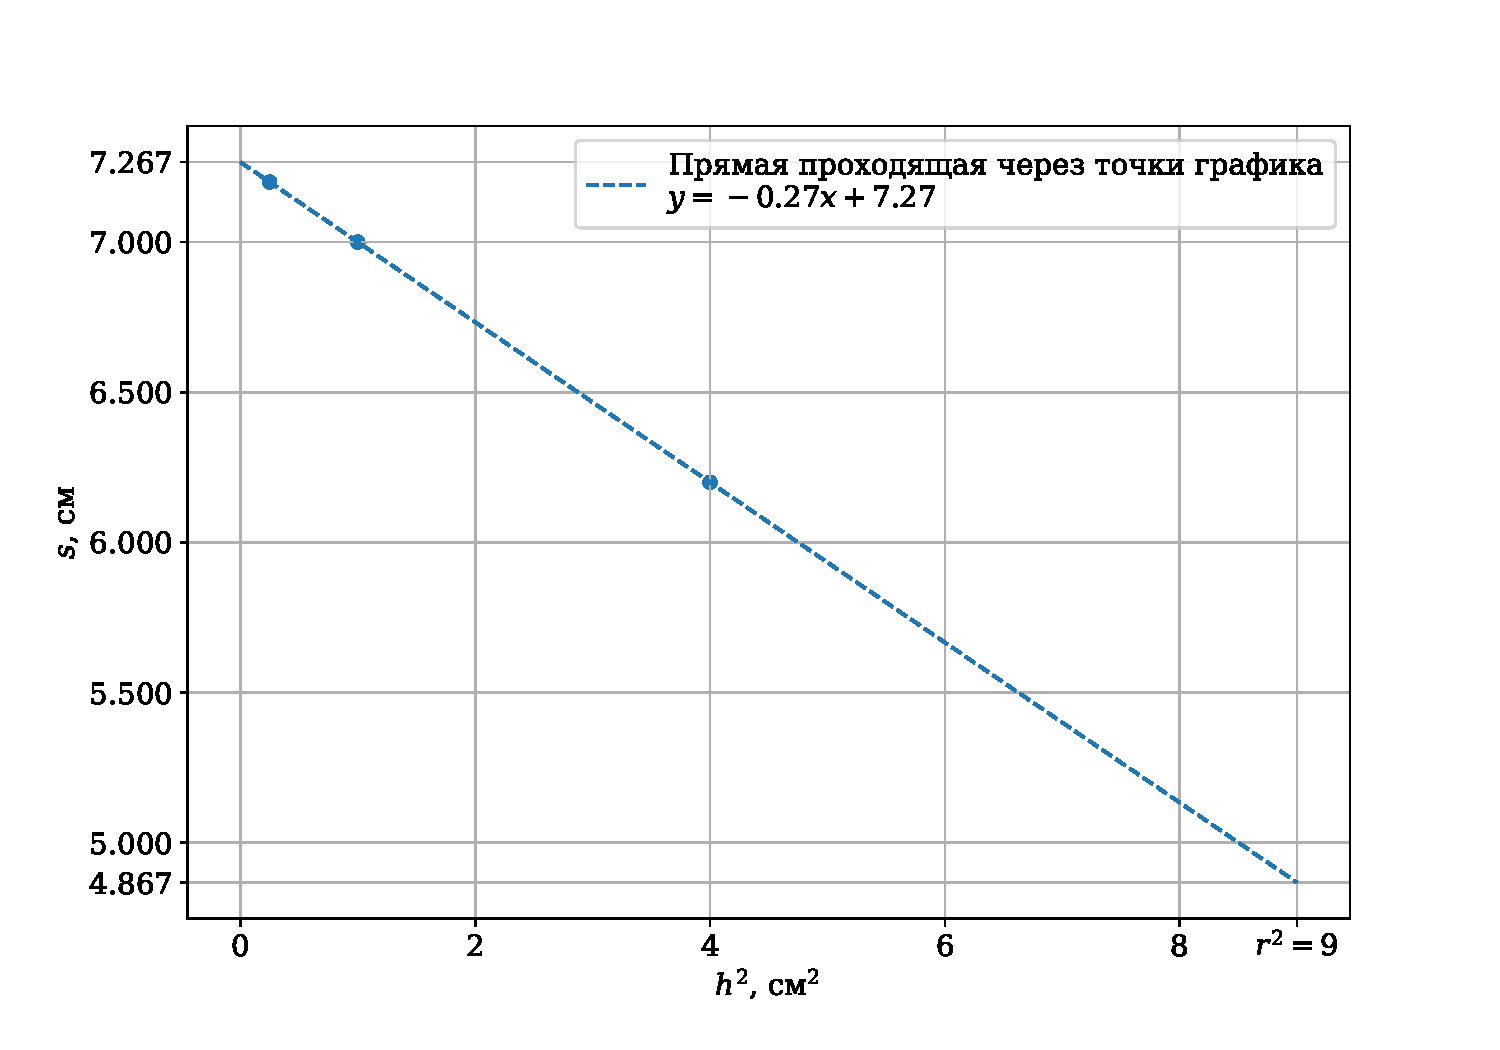
\includegraphics[width=\textwidth]{sphere.pdf}
\caption{Зависимость $s(h^2)$ для сферической аберрации}
\label{fig:shpere}
\end{figure}

\subsubsection{Хроматическая аберрация}

\paragraph{} Применяя по очереди синий, жёлтый и красный световые фильтры измерим соответствующие фокусные расстояния: $f_F = 7.4$ см, $f_D = 7$ см, $f_C = 6.5$ см. 

\paragraph{} Рассчитаем хроматическую аберрацию: $\delta f_\text{хр} = f_F - f_C = 7.4 - 6.5 = 0.9$ см и число Аббе $\nu \approx - f_D / f_\text{хр} = - 7 / 0.9 \approx - 7.8$. Значение числа Аббе получилось сильно низким, из чего можно сделать вывод, что значение хроматической аберрации завышено.

\medskip\hrule\medskip

\section{Выводы}

\begin{enumerate}
\item Измерили фокусное расстояние собирающей и рассеивающей линзы несколькими способами, за счёт чего убедились в действенности этих способов.
\item Измерили параметры сложной оптической системы, и подтвердили измерения геометрическим построением и теоретическими расчётами.
\item Измерили сферическую и хроматическую аберрации линзы.
\end{enumerate}

\medskip\hrule\medskip

\end{document}
